\newpage
\section{tournesol}

% \begin{figure}[h]
%     \centering
%     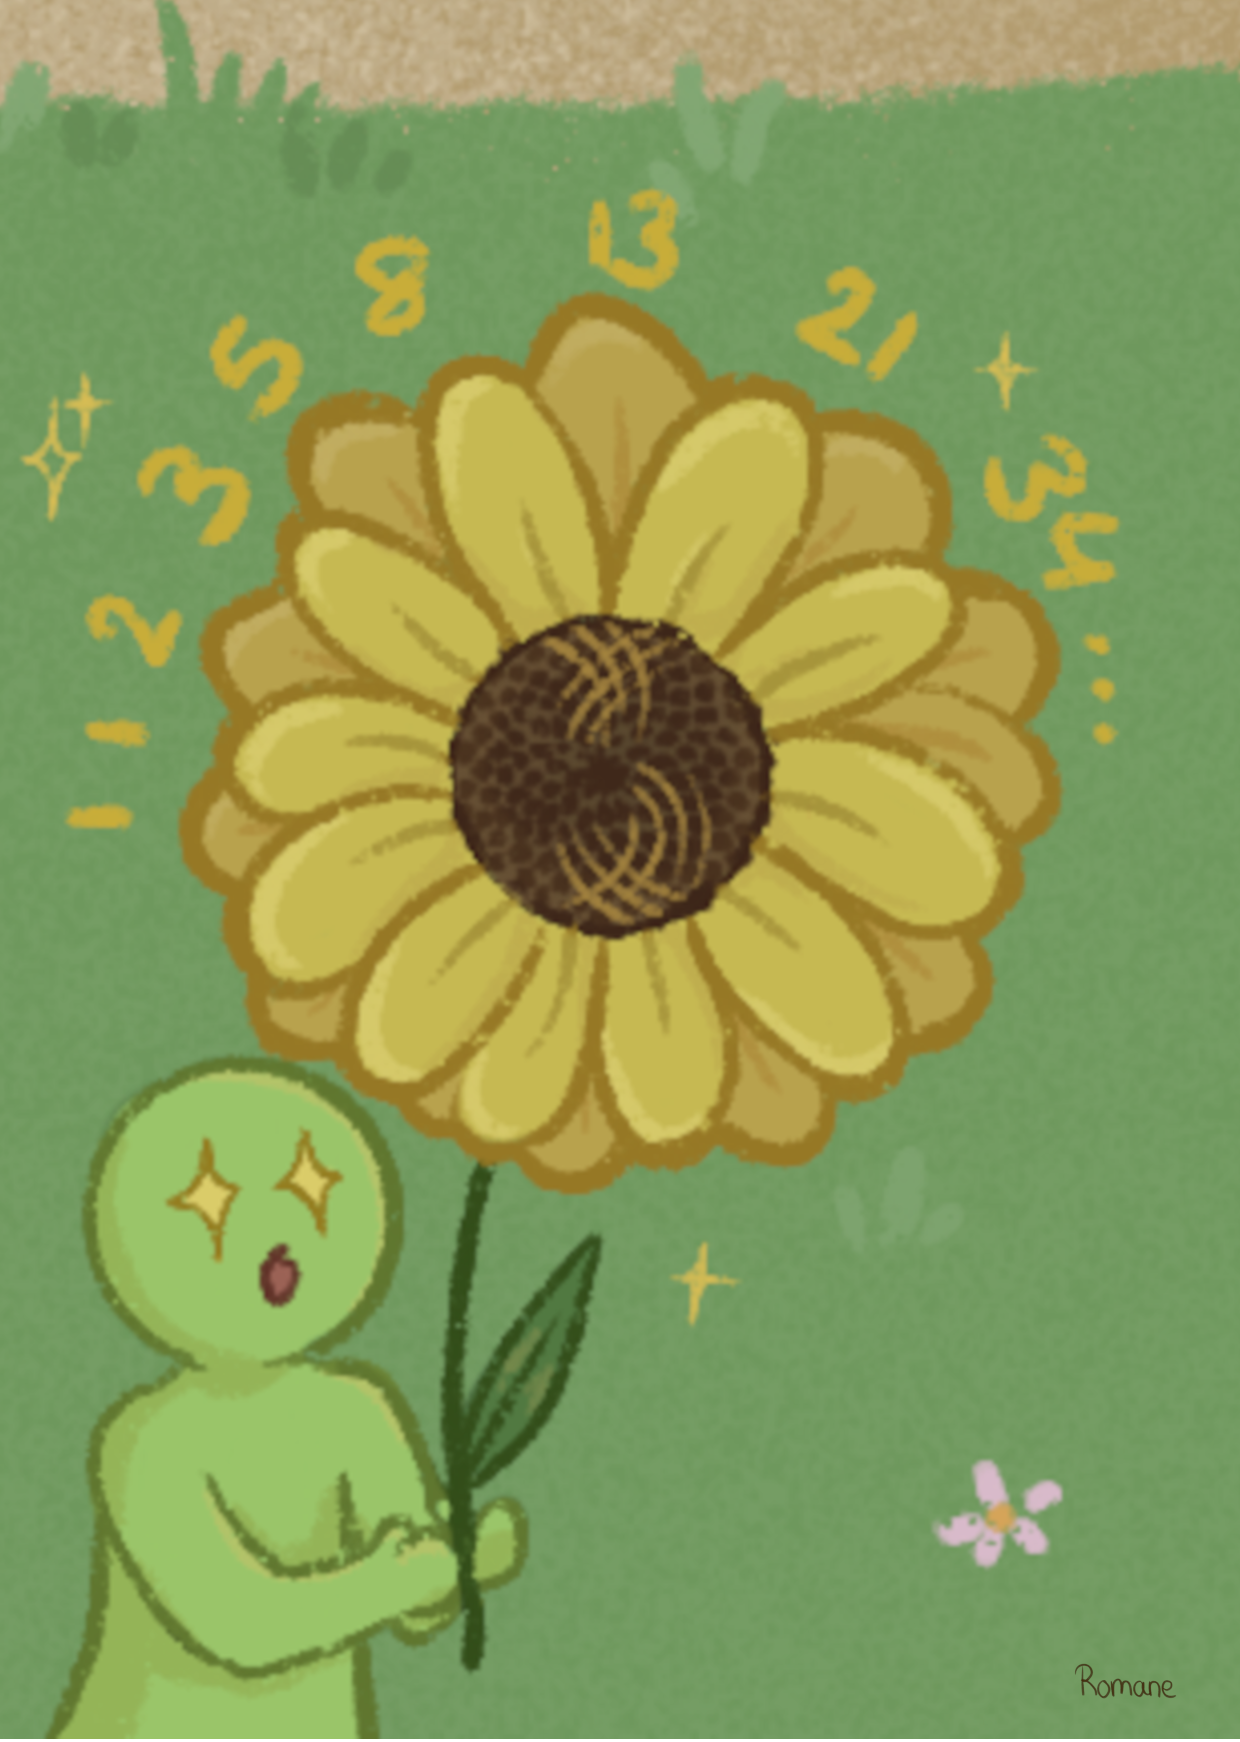
\includegraphics[height=0.5\textheight]{Cartes_postales/carte04-tournesol.png}\label{fig:c04}
%     \caption{Carte postale: Tournesol}
% \end{figure}

Les mathématiques permettent de décrire et comprendre la nature. La suite de Fibonacci est un exemple typique. C'est une suite de nombres définie de la manière suivante: les deux premiers nombres sont 0 et 1. Puis chaque nombre est obtenu en additionnant les deux précédents. Ainsi, les premiers nombres sont 0,1,1,2,3,5,8,13,21. Les termes de cette suite apparaissent dans de nombreux phénomènes de croissance dans le vivant, comme les graines de tournesol ou les formes de coquillages.

\begin{figure}[h]
    \centering
    \includegraphics[height=0.1\textheight]{Images/tournesol.png}\label{fig:c04_tournesol}
    \caption{Illustration pour différents angles}
\end{figure}

Les graines de tournesol grandissent en poussant les anciennes graines vers l'extérieur, et chaque nouvelle graine apparait depuis le centre en formant forment un angle avec les graines précédentes. Si l'angle est rationnel, par exemple 1/6, on aura 6 branches. Si l'angle vaut 11/23, on aura deux branches au début comme c'est une fraction proche de 1/2, puis on aura 23 branches. L'angle qui optimise l'espacement des graines est le nombre d'or, car c'est le plus irrationnel, et empêche les graines de s'aligner entre elles. Cet angle est très lié à la suite de Fibonnaci. On peut observer ces comportements dans le dessin ci-dessus.



\newpage
\subsection{Explications}

Les graines d'un tournesol apparaissent successivement à partir du centre de la fleur. Au fur et à mesure que les nouvelles graines apparaissent, elles repoussent les plus anciennes vers l'extérieur. Chaque nouvelle graine forme un angle avec la précédente, appelé angle de divergence. Afin de maximiser l'espacement des graines, il faut choisir un angle de divergence précis.

Si l'on choisit un angle rationnelle, par exemple un tiers de tour complet, la quatrième graine se retrouve dans l'axe de la première après trois itérations. En se poussant mutuellement, les graines finissent par former trois lignes droites. Cette structure est très inefficace car il y a beaucoup d'espace non utilisé. Ce phénomène se produit avec l'ensemble des nombres rationnels puisque, après un ou plusieurs tours complets (selon le numérateur), la structure se confronte à ce même problème d'alignement.

Il est donc plus avantageux pour la plante de prendre un nombre irrationnel comme l'angle de divergence. Pour éviter la formation de lignes, même légèrement courbées, on peut  choisir un nombre difficilement approximable par des fractions rationnelles. En mathématiques, le nombre le plus difficile à approcher par des nombres rationnels est le nombre d'or, en raison de son développement en fraction continue. C'est précisément cette proportion que l'on retrouve dans la construction des spirales de Fibonacci.

Avec cet angle spécifique, les graines ne forment jamais de lignes. Le développement des nouvelles graines engendre des spirales de Fibonacci et assure une répartition très homogène.

Image prise en utilisant https://sorciersdesalem.math.cnrs.fr/SpiralesFibo/spirale.html